% Node-link sketch of the null graphs used in BINN "real vs random" studies.
% Build: pdflatex null-graphs.tex && pdftocairo -png -r 300 -transp -singlefile null-graphs.pdf null-graphs
\documentclass[tikz,border=4pt]{standalone}
\usepackage[default]{sourcesanspro}
\usepackage[T1]{fontenc}
\usetikzlibrary{arrows.meta}

\definecolor{gene}{HTML}{9CC3E6}
\definecolor{pw}{HTML}{2A78D6}
\definecolor{root}{HTML}{1C3D6E}
\definecolor{hub}{HTML}{EB6834}
\definecolor{edge}{HTML}{8C8C8C}
\definecolor{txt}{HTML}{1C3D6E}

\tikzset{
  n/.style={circle, draw=white, line width=0.8pt, minimum size=13pt, inner sep=0pt},
  g/.style={n, fill=gene}, p/.style={n, fill=pw}, r/.style={n, fill=root},
  hub/.style={n, fill=hub},
  orphan/.style={n, fill=white, draw=edge!70, dashed, line width=0.7pt},
  e/.style={draw=edge, line width=0.9pt},
  eh/.style={draw=hub, line width=1.3pt},
  gone/.style={draw=edge!55, line width=0.8pt, dash pattern=on 1.5pt off 2pt},
}

% \panel{x offset}{title}{subtitle}{gene->pathway edges}{pathway->root edges}{orphans}{deleted edges}
% edges as a/b pairs, e.g. 1/1 = gene 1 -> pathway 1
\newcommand{\panel}[7]{
  \begin{scope}[xshift=#1cm]
    \foreach \i in {1,...,6} \coordinate (g\i) at ({(\i-3.5)*0.62}, 0);
    \foreach \j in {1,2,3} \coordinate (p\j) at ({(\j-2)*1.05}, 2.1);
    \foreach \k in {1,2} \coordinate (r\k) at ({(\k-1.5)*1.3}, 4.2);
    \foreach \a/\b in {#7} \draw[gone] (g\a) -- (p\b);
    \foreach \a/\b in {#5} \draw[e] (p\a) -- (r\b);
    \foreach \a/\b in {#4} {
      \ifnum\a=3 \draw[eh] (g\a) -- (p\b); \else \draw[e] (g\a) -- (p\b); \fi
    }
    \foreach \i in {1,2,4,5,6} \node[g] at (g\i) {};
    \node[hub] at (g3) {};
    \foreach \i in {#6} \node[orphan] at (g\i) {};
    \foreach \j in {1,2,3} \node[p] at (p\j) {};
    \foreach \k in {1,2} \node[r] at (r\k) {};
    \node[font=\bfseries\Large, text=txt, anchor=base] at (0,-1.05) {#2};
    \node[font=\large, text=edge!80!black, anchor=north, align=center] at (0,-1.3) {#3};
  \end{scope}
}

\begin{document}
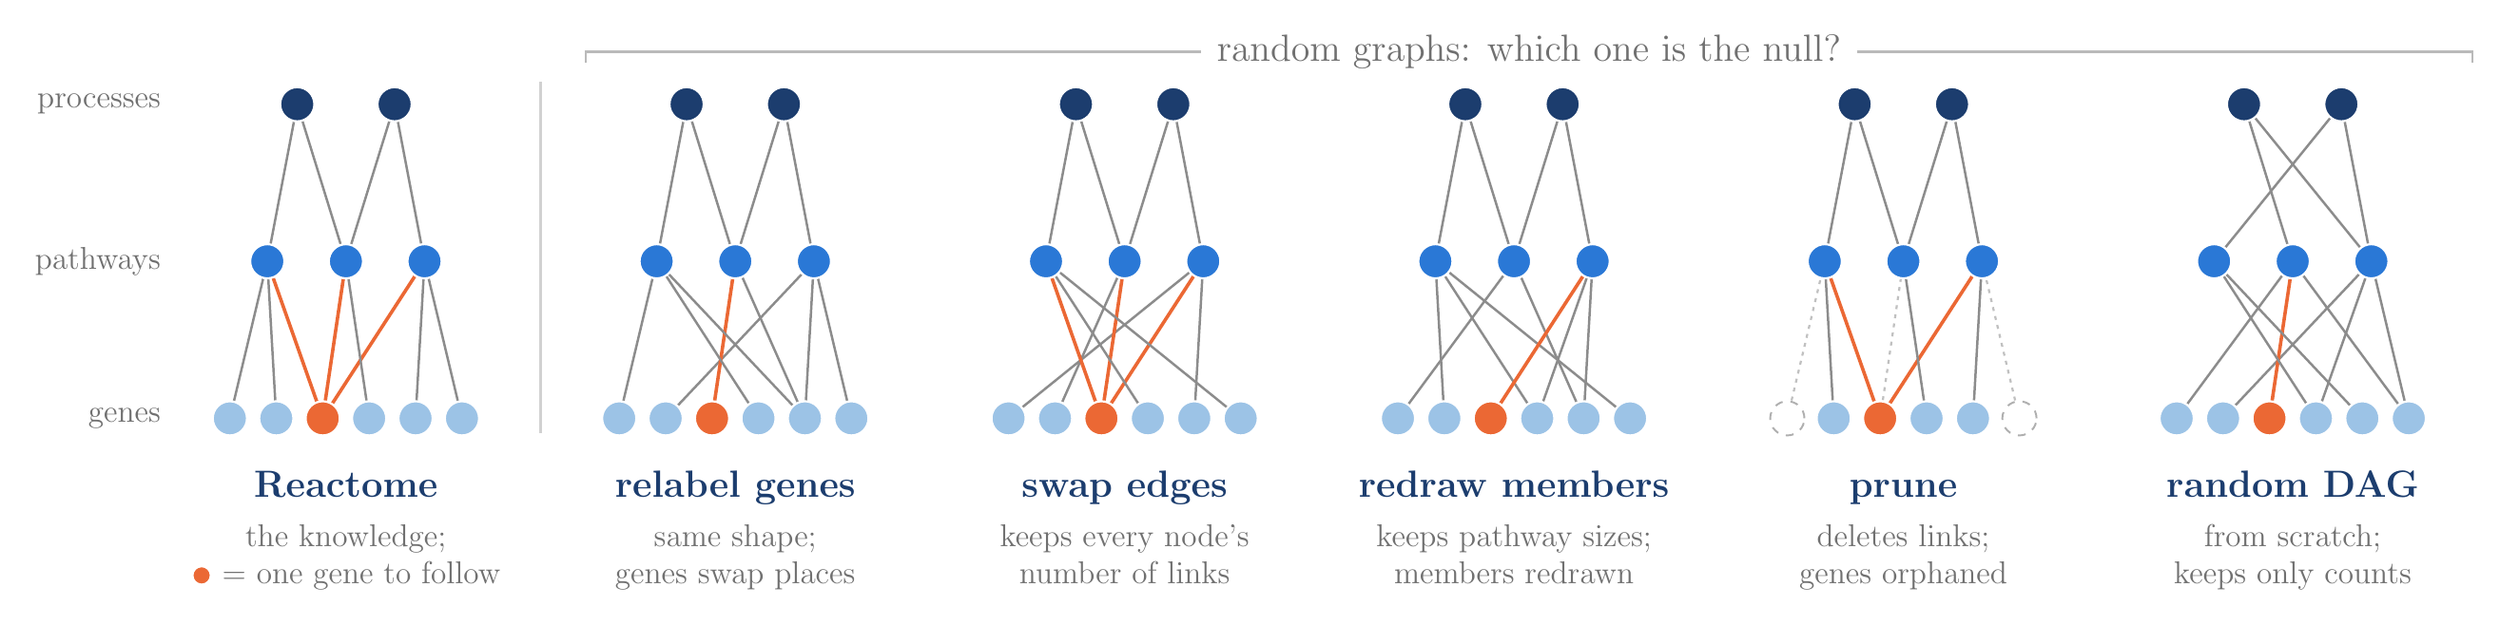
\begin{tikzpicture}
  % layer labels
  \node[anchor=east, font=\large, text=edge!80!black] at (-2.35, 0) {genes};
  \node[anchor=east, font=\large, text=edge!80!black] at (-2.35, 2.1) {pathways};
  \node[anchor=east, font=\large, text=edge!80!black] at (-2.35, 4.2) {processes};

  \panel{0}{Reactome}{the knowledge;\\\tikz[baseline=-0.6ex]\fill[hub] circle (3.5pt); = one gene to follow}
    {1/1, 2/1, 3/1, 3/2, 3/3, 4/2, 5/3, 6/3}{1/1, 2/1, 2/2, 3/2}{}{}

  \panel{5.2}{relabel genes}{same shape;\\genes swap places}
    {1/1, 2/3, 3/2, 4/1, 5/1, 5/2, 5/3, 6/3}{1/1, 2/1, 2/2, 3/2}{}{}

  \panel{10.4}{swap edges}{keeps every node's\\number of links}
    {1/3, 2/2, 3/1, 3/2, 3/3, 4/1, 5/3, 6/1}{1/1, 2/1, 2/2, 3/2}{}{}

  \panel{15.6}{redraw members}{keeps pathway sizes;\\members redrawn}
    {2/1, 4/1, 6/1, 1/2, 5/2, 3/3, 4/3, 5/3}{1/1, 2/1, 2/2, 3/2}{}{}

  \panel{20.8}{prune}{deletes links;\\genes orphaned}
    {2/1, 3/1, 3/3, 4/2, 5/3}{1/1, 2/1, 2/2, 3/2}{1,6}{1/1, 3/2, 6/3}

  \panel{26.0}{random DAG}{from scratch;\\keeps only counts}
    {1/2, 2/3, 3/2, 4/1, 4/3, 5/1, 6/2, 6/3}{1/2, 2/1, 3/1, 3/2}{}{}

  % bracket over the nulls
  \draw[edge!60, line width=0.8pt] (3.2, 4.75) -- (3.2, 4.9) -- (28.4, 4.9) -- (28.4, 4.75);
  \node[fill=white, font=\Large, text=edge!80!black, inner xsep=6pt] at (15.8, 4.9) {random graphs: which one is the null?};
  % separator after the real graph
  \draw[edge!40, line width=0.8pt] (2.6, -0.2) -- (2.6, 4.5);
\end{tikzpicture}
\end{document}
